\section{Implementation}

Based on the multiple image stereopsis observed in insects, the proposed image sensor will consist
of \(7\) hexagonal sensing areas, arranged in a honeycomb pattern. This arrangement will lead, in
the base case, to \(3\) distinct opposite image pairs, on which disparity based depth perception 
algorithms can be applied. On top of this, the sensing areas can be combined in larger resolution
sensors, with the amount of images captured changing based on the accuracy needs of the application.

\subsection*{2-dimensional sensor}

In this particular case, the honeycomb pattern is flat, allowing for classical silicon-based image
sensors to be used. The processing system will revolve around disparity map processing, using the 
center image as an anchor for the \(3\) pairs of disparity images resulted from opposite sided pairs,
highlighted in~\ref{fig2DModel}:

\begin{figure}[h]
    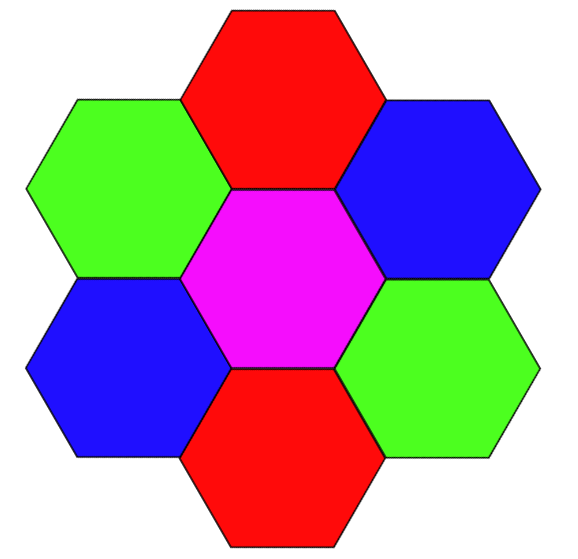
\includegraphics[width=0.50\textwidth, height=0.50\textwidth]{resources/png/2d_model.png}
    \caption{Proposed 2-dimensional model.~\label{fig2DModel}}
\end{figure}

The advantage of this system is that it can be rotated based such that the disparity axes match the 
configuration of any given scene. At the same time, the rotation can be done between two different
shots, and superposed using the center section as an anchor between the images. For determining
the depth data, an enhanced disparity map processing algorithm should be chosen, as the distance between
the image projections is identical to the size of the viewport. For this, an adaptive thresholding
algorithm, such as the one proposed by~\cite{withMain} can be used, skipping the horizontal and 
vertical enhancement steps, as they can be compensated by the other disparity pairs.

\subsection*{3-dimensional concept}

Inspired by the soft biometric device proposed by~\cite{withHexagons}, this approach will also revolve
around the use of a hemispherical image sensor, using the same \(MoS_{2}\) and graphene combination in
order to yeld significant photosensitive properties, while allowing for a structure that will not be 
damaged by the required bends.

\begin{figure}[t]
    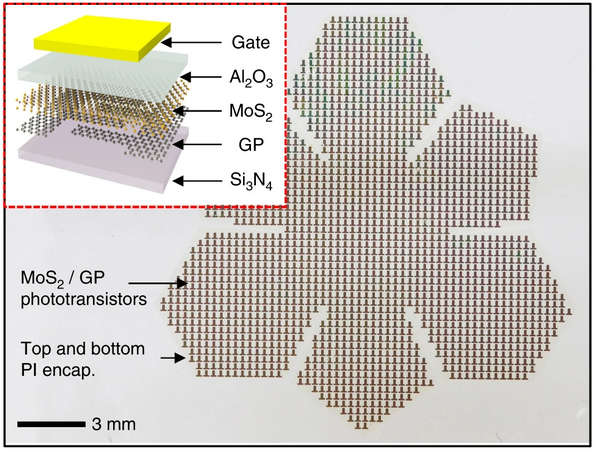
\includegraphics[width=0.50\textwidth, height=0.45\textwidth]{resources/png/paper_sensor.png}
    \caption{Phototransistor array.~\cite{withHexagons}~\label{figPaperSensor}}
\end{figure}

As shown in~\ref{figPaperSensor}, the sensor introduced by~\cite{withHexagons} represents \(7\) sides
of a truncated icosahedron, as their application required for all the sides to come together in a
seamless fashion, such that it could be used as a retinal implant. For the purposes of depth perception,
each sensing area will record an image of the same target area, therefore seams will not present an issue
in the sensor design. As such, the following honeycomb hemisphere pattern can be used:

\begin{figure}[t]
    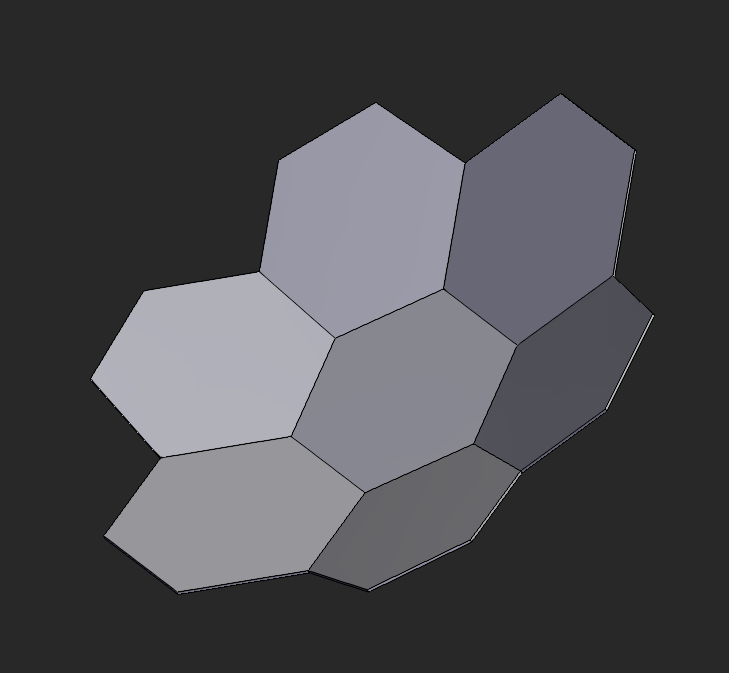
\includegraphics[width=0.50\textwidth, height=0.50\textwidth]{resources/png/3d_model.png}
    \caption{Proposed 3-dimensional model.~\label{fig3DModel}}
\end{figure}

In order to obtain the disparity data between each sensor pairs, the phase shift between the image planes
needs to be accounted for. This shift allows for more significant disparity values, as well as increasing 
the field-of-view of the resulting image. As in the case of the 2-dimensional sensor, the center area
is chosen as an anchor, with the 3-dimensional profiles being ``stitched'' on it, creating a panoramic
effect. In this case, instead of opposite sections being compared for determining the disparity images,
each area is instead compared against the center, considered the ``frontal'' view.

\subsection*{Area combination}

In particular cases, the system can be configured such that more sensing areas are used in order to record
the same image. Best used for the 2-dimensional system, as the 3-dimensional one will be affected by the 
seams between the sensing areas, this procedure can create various patterns based on the scene requirements.

\begin{figure}[t]
    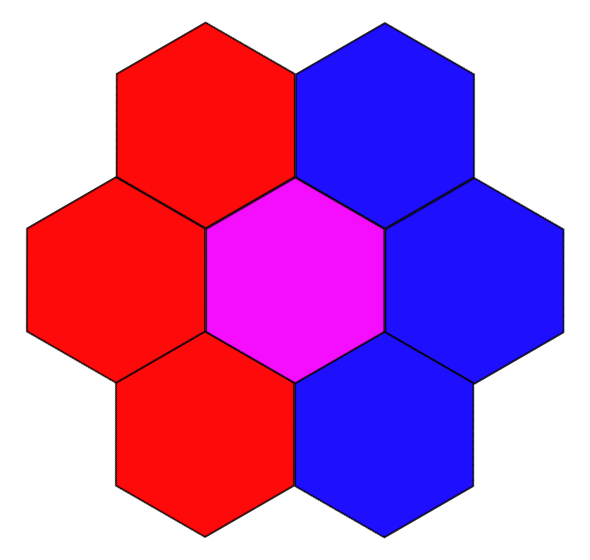
\includegraphics[width=0.50\textwidth, height=0.50\textwidth]{resources/png/stereopsis.png}
    \caption{Classical stereopsis arrangement.~\label{figStereopsis}}
\end{figure}

For example, showcased in~\ref{figStereopsis} is the recreation of classical stereopsis, using the honeycomb 
pattern. The two halves act as individual cameras, with the center section being used in order to overlap 
the end result, after the disparities are computed. As mentioned previously, coupled with the ability
to rotate the sensor around the center area, those arrangements lead to 